\begin{question}
\noindent For a Model United Nations science and culture exhibition, a student designs two similar spherical globe models to represent Earth at different scales for a UI/UX display stand.

\begin{center}
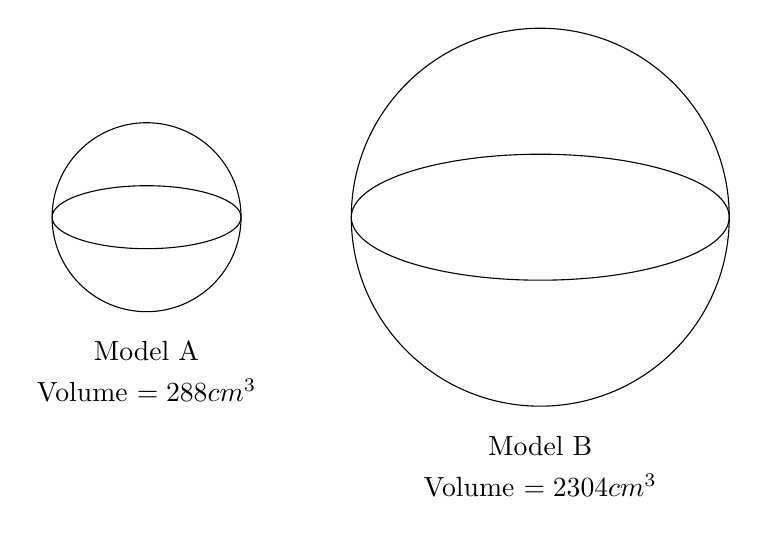
\begin{tikzpicture}[scale=1]
    % Small sphere
    \draw (0,0) circle (1.2cm);
    \draw (0,0) ellipse (1.2cm and 0.4cm);
    \node at (0,-1.7) {Model A};
    \node at (0,-2.2) {Volume $= 288\text{ cm}^3$};

    % Large sphere
    \draw (5,0) circle (2.4cm);
    \draw (5,0) ellipse (2.4cm and 0.8cm);
    \node at (5,-2.9) {Model B};
    \node at (5,-3.4) {Volume $= 2304\text{ cm}^3$};
\end{tikzpicture}
\end{center}

\noindent Model A and Model B are mathematically similar solids.

Model A has a volume of $288$ cm$^3$ and Model B has a volume of $2304$ cm$^3$.

Find the linear scale factor from Model A to Model B.

\vspace{4cm}
\answerplain{3}
\end{question}
